\documentclass{beamer}

\usepackage[utf8]{inputenc} % LaTeX, comprends les accents !
\usepackage[T1]{fontenc}     % Police contenant les caractères français
\usepackage[francais]{babel}  % Placez ici une liste de langues, la
\begin{document}

\title{Génération de traces GPS (2/2)}   
\author{Christophe Cordero \& Marc Heinrich} 
\date{\today} 

\frame{\titlepage} 

%\frame{\frametitle{Table of contents}\tableofcontents} 
\setbeamertemplate{blocks}[rounded][shadow=true]

\section{} 
\subsection{}
\frame{

\frametitle{Intérêts des traces GPS} 
\framesubtitle{} 
Agence d'urbanisme (Lyon) : \textit{Analyse de la mobilité par suivie GPS}.\\
$\Rightarrow$ équité des déplacements entre hommes et femmes.\\
$\Rightarrow$ 5 fois plus de parcours pour les parents.\\
$\Rightarrow$ ...

}

\section{} 
\subsection{}
\frame{

\frametitle{Projet commun (1/2) et (2/2)} 
\framesubtitle{Création d'un modèle} 

\begin{block}{Entrées :}
Description d'un lieu : population, carte, bâtiments, ... 
\end{block}

\vspace{\baselineskip}

\begin{block}{Sorties :}
Déplacements d'un individu véhiculé.\\
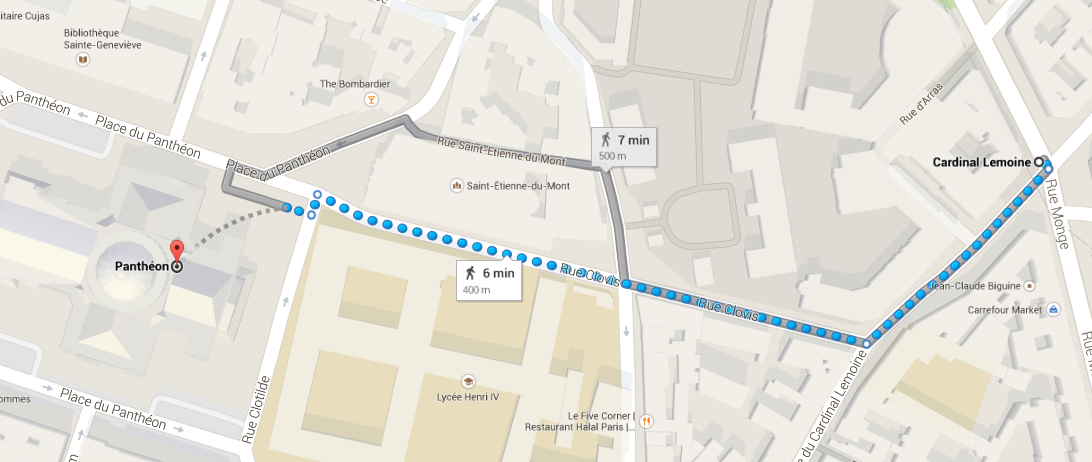
\includegraphics[scale=0.25]{ulm}\\
\end{block}


}

\section{} 
\subsection{}
\frame{

\frametitle{Plan du projet} 
\framesubtitle{Partie 2/2} 

\begin{block}{Entrées : listes d'événements}
Événement : points de départ et d'arrivée approximatifs, véhicule, date de début et de fin.
\end{block}

\onslide<2>
\begin{block}{Programme :}
\begin{itemize}
\item Calcul des bâtiments les plus proches des événements.\\
\item Calcul d'un chemin (Dijkstra) véhiculé pour chaque événements.\\
\item Temporaliser les chemins.\\
\item Bruiter (gaussien) les chemins.
\end{itemize}

\end{block}
\onslide<1,2>
\begin{block}{Sorties : chemins (GPX)}
Trace GPS qui respecte les contraintes liées à la carte et aux véhicules.
\end{block}
}

\section{} 
\subsection{}
\frame{

\frametitle{Bâtiment le plus proche} 
\framesubtitle{Données des cartes OpenStreetMap} 

\begin{center}
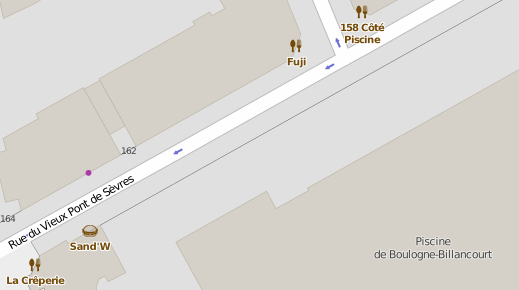
\includegraphics[scale=0.4]{donnees}\\
\end{center}
\vspace{\baselineskip}
\begin{block}{Format de données : clé $\rightarrow$ valeur}
Bâtiment $\rightarrow$ Piscine\\
Bâtiment $\rightarrow$ Restaurant
\end{block}

}

\section{}
\subsection{}
\frame{ 
\frametitle{Calcul des chemins} 
\framesubtitle{Graphhopper}
\begin{block}{Graphhopper}
Dijkstra.\\
Différents véhicules : pieds, vélo, voiture.
\end{block}
\vspace{0.5\baselineskip}
\begin{block}{Contributions}
Création d'un véhicule ferré (RER, métro, train, ...).\\
Bruitage gaussien des chemins.
\end{block}
\vspace{0.5\baselineskip}
\begin{block}{Problème}
Dépassement de mémoire (32 bits) pour 4 véhicules.
\end{block}

}

\section{}
\subsection{}
\frame{ 
\frametitle{Bruitage} 
\framesubtitle{Exemple} 
\begin{center}
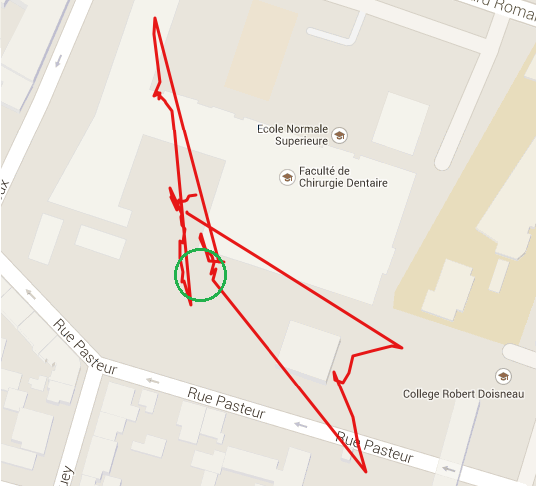
\includegraphics[scale=0.4]{bruit}\\
\end{center}
}

\section{}
\subsection{}
\frame{ 
\frametitle{Ajout d'un véhicule} 
\framesubtitle{} 
\begin{itemize}
\item première passe : déterminer les noeuds utiles
\vspace{\baselineskip}
\item deuxième passe : calculer les vitesses
\vspace{\baselineskip}
\item problème : déterminer exactement quels noeuds prendre
\end{itemize}
\vspace{\baselineskip}
}


\section{}
\subsection{}
\frame{ 
\frametitle{Démonstration} 
\framesubtitle{}
. Codé en Java.\\
\vspace{\baselineskip}
. Librairies utilisées :\\
- Osmosis (traitement des données OSM)\\
- Graphhopper\\
\vspace{\baselineskip}
. Projet : https://github.com/mheinric/projectWebdata
}


\end{document}

